\section{Architecture}
\label{sec:architecture}

An application for the analysis of evolving criminal networks requires the real-time processing of heterogeneous data from multiple distributed data sources.
%
%In an widely extended criminal scenario, the amount of data is huge, heterogeneous and generated rapidly. 
To extract valuable information from these data sources, the system must be highly scalable, provide high throughput, and allow a convenient exploration of results.
%: a large number of people, criminals, devices, and sensors are connected via digital networks, and their interactions generate enormous valuable information \cite{FrameworkBigdata}. For these reasons, we are interested to an high-throughput and scalable process of analysis.
%Furthermore, application usage as a tool to support the law enforcement agencies, it requires the storage capacity of the social network in a database that can be consulted rapidly.

Considering these requirements, we propose an application that follows the 
% \textit{data stream processing} (DSP) 
DSP approach. 
A DSP application is modeled as a graph of connected operators, where each one implements a task to be executed on-the-fly on continuous streams of data.

Our application provides an extremely flexible architecture, making it really easy to deploy and evaluate performances of any metric.
It provides high scalability and throughput 
% leveraging 
(i) by decoupling the elaboration steps of data injection, data processing, and data storage, 
(ii) by distributing stateless DSP operators to improve performance and independence of their evolution over time,
(iii) by adapting a highly scalable publish/subscribe system 
(iv) by adopting a high-throughput DSP framework,
and (v) by leveraging on a graph-based storage system, optimized for read-intensive tasks.

In Figure~\ref{fig:topology_layered}, we show the layered architecture of the application. The data stream processing core is implemented with \textit{Apache Flink} \cite{flink}, a highly scalable DSP framework notable for its throughput maximisation.
Data injection is provided by \textit{Apache Kafka} \cite{kafka}, a widely adopted pub/sub system natively thought to implement asynchronous communication in big data analytics applications.
Criminal network graph is stored in \textit{Neo4j} \cite{neo4j}, a highly scalable graph database that optimises the storage of large graphs and provides a convenient web-based data exploration tool.

\begin{figure}
\centering
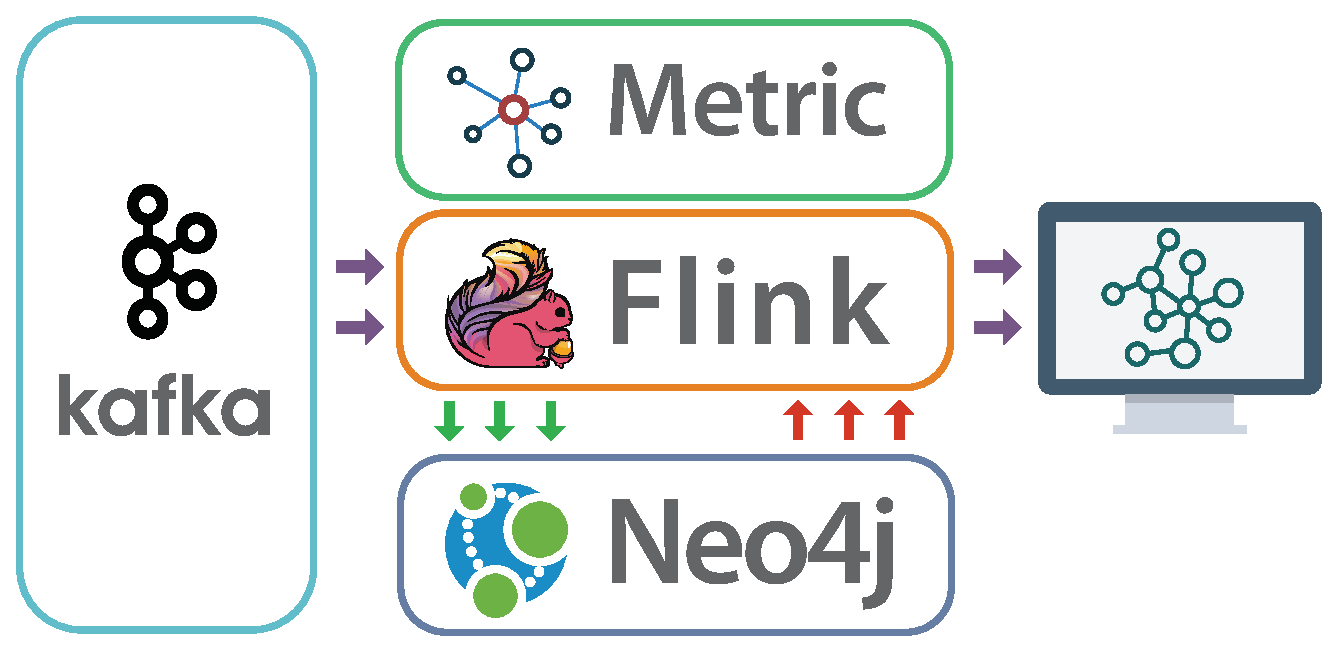
\includegraphics[width=2.5in]{./fig/crimegraph-layered-architecture}
\caption{The layered architecture}
\label{fig:topology_layered}
\end{figure}

In Figure~\ref{fig:topology}, we represent the architecture of the proposed application, with a focus on the topology of stream operators. Data coming from heterogeneous sources are injected into the system with Kafka. The \texttt{GraphUpdate} operator records the received interactions into Neo4j, triggering accordingly an update of the criminal network.
The \texttt{ScoreCalculator} operator computes the deployed metrics retrieving from Neo4j the required features of the criminal network. The links with the score previously computed are then split into hidden and potential links, from which are filter out those that are under the given threshold.
The evolving graph made of real and mined links can be visualized and explored with the Neo4J Web Browser.

\begin{figure*}
\centering
\includegraphics[width=7.1in]{./fig/topology}
\caption{The architecture.}
\label{fig:topology}
\end{figure*}
